\newpage
\section*{B: ABC analysis method}
    \phantomsection\addcontentsline{toc}{subsection}{\numberline {}B. ABC analysis method}
    \label{apx:B}

Prior to laying out a warehouse, deciding on the most appropriate handling equipment, installing storage systems and deciding on which form of picking system to introduce, a full ABC analysis of stock movements and stock held should take place.

Understanding ABC classification begins by understanding Pareto's Law or the 80/20 rule. Pareto's Law is widely used in logistics and is an excellent method for categorizing items. This is normally termed ABC classification.

It is states that roughly 80 percent of effects come from 20 percent of
causes. This rule is not universal but it is surprising how often it can apply. The idea therefore is to concentrate time and resources on the important 20 percent or the 'vital few'.

    \begin{figure}[!ht]
        \centering
        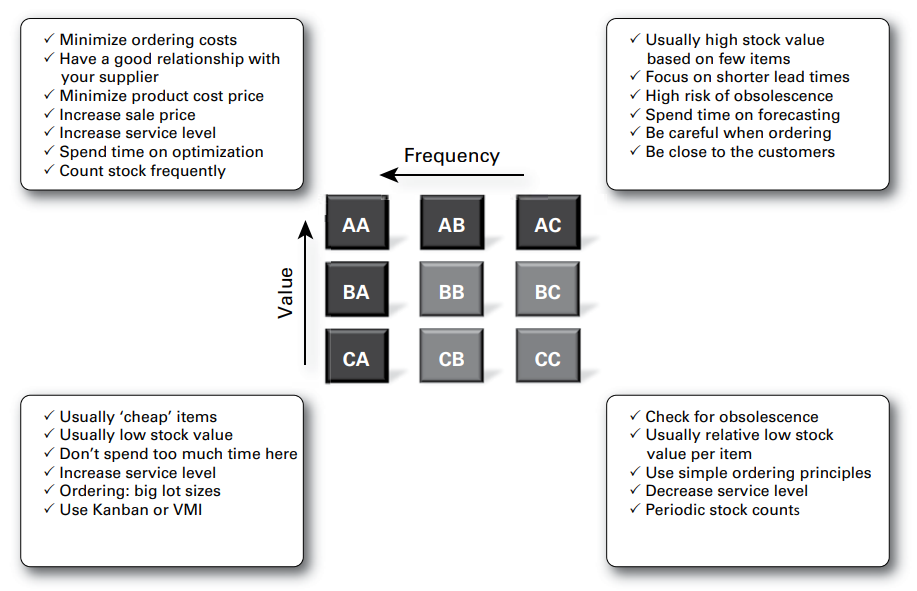
\includegraphics[width=16cm,height=11cm]{figure/abc.png}
        \caption{ABC analysis: product value and frequency of sales}
        \label{fig:abc}
    \end{figure}
